\subsection{Chain of Responsibility}
\begin{flushleft}
	\textbf{Chain of Responsibility} là một mẫu thiết kế hành vi (behavioral design pattern) cho phép bạn truyền yêu cầu qua một chuỗi các bộ xử lý (handlers). Khi nhận được một yêu cầu, mỗi bộ xử lý sẽ quyết định hoặc xử lý yêu cầu đó hoặc chuyển nó cho bộ xử lý tiếp theo trong chuỗi.
\end{flushleft}

\subsubsection{Vấn đề}
\begin{flushleft}
	\begin{itemize}
		\item \textbf{Xử lý yêu cầu phức tạp:} Khi một yêu cầu cần được xử lý qua nhiều giai đoạn khác nhau, việc quản lý luồng xử lý và các điều kiện chuyển tiếp giữa các giai đoạn có thể trở nên phức tạp.
		\item \textbf{Mở rộng hệ thống:} Khi cần thêm hoặc xóa các giai đoạn xử lý, việc sửa đổi toàn bộ hệ thống có thể gây ra nhiều rắc rối.
		\item \textbf{Tách biệt mối quan tâm:} Các logic xử lý khác nhau được phân tán vào các lớp khác nhau, giúp code dễ đọc và bảo trì hơn.
	\end{itemize}
\end{flushleft}

\subsubsection{Mục đích}
\begin{flushleft}
	\begin{itemize}
		\item \textbf{Tách biệt các bước xử lý:} Mỗi bước xử lý được đóng gói trong một đối tượng riêng biệt (handler).
		\item \textbf{Xử lý theo chuỗi:} Các handler được liên kết thành một chuỗi, yêu cầu sẽ được truyền qua chuỗi cho đến khi được xử lý hoặc đạt đến cuối chuỗi.
		\item \textbf{Linh hoạt:} Dễ dàng thêm, xóa hoặc thay đổi thứ tự các handler mà không ảnh hưởng đến các phần còn lại của hệ thống.
	\end{itemize}
\end{flushleft}

\subsubsection{Giải pháp}
\begin{flushleft}
	\begin{itemize}
		\item Giống như nhiều mẫu thiết kế hành vi khác, \textit{Chain of Responsibility} dựa trên việc biến đổi các hành vi cụ thể thành các đối tượng độc lập gọi là \textit{handlers}.
		\item Mỗi công đoạn nên được trích xuất thành một lớp riêng biệt với một phương thức duy nhất thực hiện hành động cụ thể theo từng công đoạn. Yêu cầu, cùng với dữ liệu của nó, được truyền vào phương thức này như một đối số
		\item Mỗi handler được liên kết có một trường để lưu trữ tham chiếu đến handler tiếp theo trong chuỗi. Ngoài việc xử lý yêu cầu, các handlers còn truyền yêu cầu tiếp tục dọc theo chuỗi. Yêu cầu di chuyển dọc theo chuỗi cho đến khi tất cả các handlers đều có cơ hội xử lý nó.
	\end{itemize}
\end{flushleft}

\subsubsection{Cấu trúc}
\begin{flushleft}
	\begin{itemize}
		\item \textbf{OrderHandler:} Giao diện chung cho tất cả các handler, định nghĩa hai phương thức chính:
		      \begin{itemize}
			      \item \verb|setNext|: Thiết lập handler tiếp theo trong chuỗi.
			      \item \verb|handle|: Xử lý yêu cầu.
		      \end{itemize}
		\item \textbf{BaseHandler:} Lớp trừu tượng triển khai giao diện \verb|OrderHandler|, cung cấp một thuộc tính \verb|next| để lưu trữ handler tiếp theo.
		\item \textbf{SelectItemStage, AddressInfoStage, PaymentStage, ShippingStage, CompletionStage:} Các lớp cụ thể kế thừa từ \verb|BaseHandler|, đại diện cho các giai đoạn xử lý khác nhau trong một đơn hàng. Mỗi giai đoạn sẽ thực hiện một nhiệm vụ cụ thể và quyết định có chuyển yêu cầu đến giai đoạn tiếp theo hay không.
	\end{itemize}

    \begin{figure}[H]
        \centering
        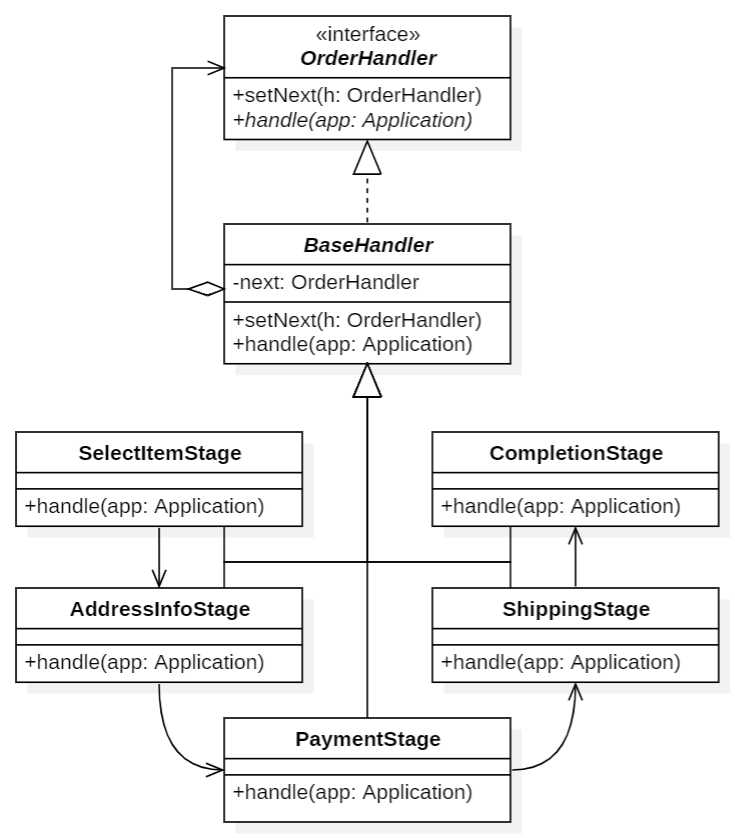
\includegraphics[width=0.9\textwidth]{../assets/screenshots/uml/cor.png}
        \caption{Chain of Responsibility UML Class Diagram}
    \end{figure}
\end{flushleft}

\subsubsection{Hoạt động}
\begin{flushleft}
	\begin{itemize}
		\item \textbf{Tạo chuỗi handler:} Các handler được khởi tạo và liên kết với nhau thành một chuỗi.
		\item \textbf{Gửi yêu cầu:} Yêu cầu được gửi đến handler đầu tiên trong chuỗi.
		\item \textbf{Xử lý yêu cầu:}
		      \begin{itemize}
			      \item Nếu handler hiện tại có thể xử lý yêu cầu, nó sẽ thực hiện các tác vụ cần thiết và dừng quá trình.
			      \item Nếu handler hiện tại không thể xử lý, nó sẽ chuyển yêu cầu đến handler tiếp theo trong chuỗi.
		      \end{itemize}
		\item \textbf{Lặp lại bước 3:} Quá trình này tiếp tục cho đến khi yêu cầu được xử lý hoặc đạt đến cuối chuỗi.
	\end{itemize}
\end{flushleft}

\subsubsection{Khả năng ứng dụng}
\begin{flushleft}
	\begin{itemize}
		\item \textbf{Xử lý đơn hàng:} \textit{CoR Pattern} được sử dụng rộng rãi trong các hệ thống xử lý đơn hàng để quản lý các giai đoạn khác nhau như thanh toán, vận chuyển.
		\item \textbf{Xử lý sự kiện:} Có thể sử dụng CoR để xử lý các sự kiện trong giao diện người dùng, chẳng hạn như các sự kiện click chuột để chuyển sang công đoạn kế.
		\item \textbf{Logging:} Mỗi handler có thể ghi lại thông tin về quá trình xử lý yêu cầu.
	\end{itemize}
\end{flushleft}

\subsubsection{Ưu nhược điểm}
\begin{enumerate}
	\item \textbf{Ưu điểm}
	      \begin{itemize}
		      \item \textbf{Linh hoạt:} Dễ dàng thêm, xóa hoặc thay đổi các handler.
		      \item \textbf{Mở rộng:} Có thể dễ dàng mở rộng hệ thống bằng cách thêm các handler mới.
		      \item \textbf{Tái sử dụng:} Các handler có thể được sử dụng lại trong các hệ thống khác.
		      \item \textbf{Giảm sự kết hợp:} Các handler không cần biết về các handler khác trong chuỗi.
	      \end{itemize}
	\item \textbf{Nhược điểm}
	      \begin{itemize}
		      \item \textbf{Khó phát hiện lỗi và debug:} Nếu chuỗi (chain) quá dài và phức tạp, việc tìm ra lỗi có thể khó khăn.
		      \item \textbf{Hiệu suất:} Nếu có quá nhiều handler, việc truyền yêu cầu qua chuỗi có thể làm giảm hiệu suất.
	      \end{itemize}
\end{enumerate}

\subsubsection{Mã nguồn}
\codeimport{cpp}{../src/ecommerce-demo/Stage.hpp}
